%%%%%%%%%%%%%%%%%%%%%%%%%%%%%%%%%%%%%%%%%
% Large Colored Title Article
% LaTeX Template
% Version 1.0 (15/8/12)
%
% This template has been downloaded from:
% http://www.LaTeXTemplates.com
%
% Original author:
% Frits Wenneker (http://www.howtotex.com)
%
% License:
% CC BY-NC-SA 3.0 (http://creativecommons.org/licenses/by-nc-sa/3.0/)
%
%%%%%%%%%%%%%%%%%%%%%%%%%%%%%%%%%%%%%%%%%

%----------------------------------------------------------------------------------------
%	PACKAGES AND OTHER DOCUMENT CONFIGURATIONS
%----------------------------------------------------------------------------------------

\documentclass[DIV=calc, paper=a4, fontsize=11pt, twocolumn]{scrreprt}	 % A4 paper and 11pt font size

\usepackage{lipsum} % Used for inserting dummy 'Lorem ipsum' text into the template
\usepackage[english]{babel} % English language/hyphenation
\usepackage[protrusion=true,expansion=true]{microtype} % Better typography
\usepackage{amsmath,amsfonts,amsthm} % Math packages
\usepackage[svgnames]{xcolor} % Enabling colors by their 'svgnames'
\usepackage[hang, small,labelfont=bf,up,textfont=it,up]{caption} % Custom captions under/above floats in tables or figures
\usepackage{booktabs} % Horizontal rules in tables
\usepackage{fix-cm}	 % Custom font sizes - used for the initial letter in the document
\usepackage[utf8x]{inputenc}

\usepackage{sectsty} % Enables custom section titles
\allsectionsfont{\usefont{OT1}{phv}{b}{n}} % Change the font of all section commands

\usepackage{soul} % for highlighting, underlining etc.
\usepackage{hyperref} % for hyperlinks
\hypersetup{ % for colored links not in a box.
  colorlinks=true
}

\usepackage{graphicx} % for graphics
\usepackage{moreverb} % code snippets
\usepackage{float}

\usepackage{lettrine} % Package to accentuate the first letter of the text
\newcommand{\initial}[1]{ % Defines the command and style for the first letter
  \lettrine[lines=3,lhang=0.3,nindent=0em]{
    \color{DarkGoldenrod}{
      \textsf{#1}
    }
  }{}
}

%----------------------------------------------------------------------------------------
%	LAYOUT SECTION
%----------------------------------------------------------------------------------------

\usepackage{lastpage} % Used to determine the number of pages in the document (for "Page X of Total")
\usepackage{fancyhdr} % Needed to define custom headers/footers
\fancypagestyle{plain}{% Overwriting the plain, so the table of contents will use it too
  % Headers
  \fancyheadoffset{0.5 cm}
  \lhead{\nouppercase{\leftmark}}
  \chead{\textbf{A}rtificial \textbf{I}ntelligence}
  \rhead{\today}

  % Footers
  \fancyfootoffset{0.5 cm}
  \lfoot{Michael Gerber, Nicolas Ganz}
  \cfoot{}
  \rfoot{\footnotesize Page \thepage\ of \pageref{LastPage}} % "Page 1 of 2"

  \setlength{\topmargin}{-30pt}
  \addtolength{\textheight}{-40pt}
  \setlength{\columnsep}{1.5cm}
  \setlength{\columnseprule}{0.4pt}

  \renewcommand{\headrulewidth}{0.4pt} % Thin header rule
  \renewcommand{\footrulewidth}{0.4pt} % Thin footer rule
}

\pagestyle{plain}

%----------------------------------------------------------------------------------------
%	TITLE SECTION
%----------------------------------------------------------------------------------------

\usepackage{titling} % Allows custom title configuration

\newcommand{\HorRule}{\color{DarkGoldenrod} \rule{\linewidth}{1pt}} % Defines the gold horizontal rule around the title

\pretitle{
  \vspace{-30pt}
  \begin{flushleft}
    \HorRule
    \\[0.4cm]
    \fontsize{30}{30}
    \usefont{OT1}{phv}{b}{n}
    \color{DarkRed}
} % Horizontal rule before the title

\posttitle{
    \par
  \end{flushleft}
  \vskip 0.5em
} % Whitespace under the title

\preauthor{
  \begin{flushleft}
    \large
    \lineskip 0.5em
    \usefont{OT1}{phv}{b}{sl}
    \color{DarkRed}
} % Author font configuration

\postauthor{
    \footnotesize
    \usefont{OT1}{phv}{m}{sl}
    \color{Black}
    % Configuration for the institution name
    BIA 09 7b - BMS Zürich % Your institution
    \par
  \end{flushleft}
  \HorRule
} % Horizontal rule after the title


\begin{document}

\newcommand{\printhref}[2]{
  \href{#1}{#2 (#1)}
}

\begin{titlepage}
  \thispagestyle{empty}

  \title{AI applied to a simple 2D environment} % Your article title
  \author{Michael Gerber, Nicolas Ganz } % Your name
  \maketitle % Print the title
\end{titlepage}

\tableofcontents
%----------------------------------------------------------------------------------------
%	ABSTRACT
%----------------------------------------------------------------------------------------

\chapter{Abstract}
% The first character should be within \initial{}
\initial{H}\textbf{ere is some sample text to show the initial in the introductory paragraph of this template article. The color and line height of the initial can be modified in the preamble of this document.}

%------------------------------------------------
\chapter{Artificial Intelligence}
\section{What is AI?}

This question has about as many answers as there are people studying artificial intelligence. Without getting too philosophical one could say that intelligence is defined by the efficiency of patterns used to solve problems in a complex environment and the ability to learn or generate new patterns by observing or testing.

Man-made programs to solve such problems have been around for decades and as algorithm efficiency and computational power increases they get ever more powerful.

An AI usually is directed towards one goal. This could mean solving a mathematical challenge most efficiently, finding patterns in huge amounts of data to categorize new sets of data or even to find smarter ways of learning.


\section{History of the Field}

The idea of artificial creatures acting and thinking like humans has been documented as far back as ancient Egypt. But it wasn't until the year 1955 that John McCarthy used the term artificial intelligence and defined it as "the science and engineering of making intelligent machines".
Only a year later AI research became a scientific field at the campus of Dartmouth College. During the 1960s the Department of Defense was heavily funding AI research and the field was taught around the world.
For the next decades research continued with big advances in problem solving but few real world applications. In 1997 the field drew a lot of public attention after IBM's chess computer Deep Blue famously defeated the reigning world champion Garry Kasparov.
In the 21st century AI has found many applications in fields like medical diagnostics, data mining or household appliances like the "Roomba". 

\section{Technological Singularity}

\newpage
\section{Real World Applications}

Artificial Intelligence Technology 

\subsection{Amazon Recommendations}
Everyone knows the ``People who bought X also bought Y''-kind of recommendations online shops provide you with. Sometimes they are spot on and other times they are as far off as they can be. The idea of course is to find patterns in customer interest which can be used to offer people things they are likely to buy thereby increasing profit.

So how do they work? It is all about finding similarities in data. In the case of products you have attributes like cost, size, style, manufacturer, etc. that let classify the product. Yet taken for themselves they are close to useless because two products that are similar in size and cost might not have anything in common at all. It's even worse. Imagine two lamps that have almost the same price, the same size and the same style. What's the probability that someone who bought the one lamp would also want to buy the other? Close to zero. Now why is that? For one thing it's unlikely that someone needs two lamps. It's even less likely that they would need two almost identical lamps. So apart from flat stats about a product one needs to take into account the nature of the product to make good recommendations. An example of such would be matching light bulbs for the lamp. 
This tells us two things. First we need to categorize a product. Not only in it's use (e.g. lamp, chair, table, clock) but also in what frequency demand for it arises. So for example one would like to buy a new shirt every month whereas a new computer is only required every few years. The second thing is that there are certain items which depend on other items to function. A coffee machine needs filters, a toy car needs batteries and a lamp needs light bulbs. Hence to make a smart suggestion one would link those items one way so that buying a laptop would yield to recommendation of a mouse but buying cat food would not recommend acquiring a new feline companion.

This probably all sounds perfectly reasonable. Every halfway decent online shop should be capable handling categories and dependencies between products. Since the assignment of such seems more or less obvious even to an intern why not just hire some of those to do it? It doesn't require an expensive AI to figure out that it would be a good idea to recommend "Harry Potter" part two to someone who bought part one. Yet if those where to only clues to go on the list of suggestions would be pretty short for most products. To make matters worse: Since those types of relations are so obvious, it's likely the customer thought of them already so they don't yield as much additional sales as "smart" recommendations would. This is where the AI algorithms come in.

Imagine what a resale company could do if they understood their customer's taste. If they knew what style of clothing she likes, whether she lives near a beach and thus is more likely to buy a new bathing suit in spring or when her mothers birthday was so they could recommend gifts for older women at that time of year. Admittedly these examples might are little extreme yet the efforts of the so called data miners definitely go in that direction. These three examples have been picked for a reason because they each depend on different types of data.

The style for example can be derived from the clothes the customer has bought in the past. From those the retailer could categorize his customers into groups that appear to like the same products and recommend things person A from this group bought to person B. Of course there is more to it than that. For example one needs to filter out noise which may be a piece of clothing a customer bought for someone else and thus does not match the pattern. Now an especially smart AI could even make a connection between such purchases and the friend or family member they where meant to. This data then could be used for a variety of further predictions about the customers buying behavior.

The fact whether someone lives near a beach (or swimming pool for that matter) can be easily determined by matching the IP address from which requests to the store website were made to the corresponding location. There is a lot more of this type of information that one can easily read from the web request like browser type, mobile phone model, referring website and by matters of recurring visits from different locations even estimates about the customer's place of work or their boyfriend's address. Now this type of information is only as useful as one is able to make sense of it. This is the true strength of an AI because it can find patterns in data that no one has been looking for so far.

\subsection{Web Search Algorithms}

In web search it is even more important than with large selections of products to have an automated way to make precise estimations about the value of something to someone. Furthermore the search provider not only wants to establish a prediction about how likely a person is to be looking for a certain web page but also about how likely he or she is to be looking for it right now. A lot of things factor into this like previously visited websites, behavior in choosing links and probably over a thousand other data points that might have been collected about a person. Yet even if there is no previous information about a search engine user available they can still make predictions based on the location, language and outside factors. An example of this might be the following scenario:

A user sits down in a Boston coffee shop using a browser, the signature of which has been modified to prevent it from being tracked back to that certain individual, to access her search provider of choice. She types in the word "dolphins". Now the first assumptions is that she is looking for the marine mammals. Yet the night before the football team by the same name might have played which would vastly improve the relevance of last nights game results. This increase of relevance can be justified by the fact that the user has set her language preference to American English which makes it far more likely that she is interested in the score than someone with a preference for French would be. But this isn't everything that is relevant to the search. Assuming that a band called "The Dolphins" is playing this week in Boston would make the band's website and a ticket sales site a lot more relevant to this search then it would be for someone from San Francisco.

Again this example shows how a shift in relevance might be obvious if pointed out but is extremely hard to predict for a human. Artificial intelligence can look at changes in user behavior (like increased requests to "The Dolphins" band website from Boston) and smartly adjust the ranking of certain websites. Of course this is an oversimplification of the problem but it shows nicely the basic idea of using AI to find patterns in changing data.

\subsection{DARPA Challenges}

The Defense Advanced Research Projects Agency has funded prize competitions that reward advances in research fields relevant to the Department of Defense. The initial challenge was to build autonomous ground vehicles or "self-driving cars". It was called the DARPA Grand Challenge and was first held in 2004. The goal was to build an autonomous vehicle that could drive the 240 km route through the desert fastest. None of the robot vehicles that entered the contest was able to complete the challenge. The one that performed best only finished five percent of the route before getting hung up on a rock. Therefore the event was repeated in 2005.

The second time around five vehicles were able to finish the race. With the team from Stanford University finishing first. 

In 2007 the DARPA Urban Challenge has been held requiring the vehicles to finish a 96 km course in an urban area while obeying traffic regulations and interacting with human drivers.

Currently Google is developing a driverless car which has already driven 300'000 miles without an accident. The project is led by Sebastian Thrun who also was the head of the Stanford team that won the 2005 DARPA Grand Challenge.

\subsection{IBM Watson}

\section{Classification of AI problems}

There are four major attributes to an AI problem. Each of them has severe impact on how one approaches to solve that given problem.
\begin{description}
\item Firstly there is the question of observability. Some environments are {\bf fully observable} while others are only {\bf partially observable}.
\item Secondly there is the factor of randomness. An environment can be completely {\bf deterministic} which means that taking an action always result in the expected state or {\bf stochastic}. In the latter case there is chance involved in determining the outcome of an action. A good example for this would be a game that requires one to roll dice.
\item Thirdly a problem might either be {\bf discrete} or {\bf continuous}. The former one meaning that there is a finite number of things to do and things to observe and the latter meaning that there is a factor to the problem that is infinite and has to be handled accordingly.
\item Fourthly the problems environment can be {\bf benign} or {\bf adversarial} which would mean that there are factors to it that are actively contradicting the AI's objective by taking actions that prevent it from achieving its goals. Most games are of adversarial nature because in order to succeed each player needs to take actions that make it harder for his opponents to win.
\end{description}

\newpage
\section{Important AI Algorithms in Detail}
\subsection{Tree Search}

In artificial intelligence many problems can be represented as trees. The first node of that tree is the initial state of the problem. From that state different actions can be taken which lead to new states. A good example of this is the game of Tic Tac Toe.

\begin{figure}[H]
  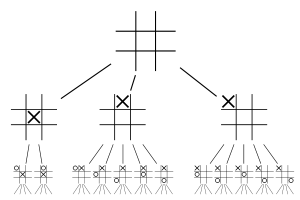
\includegraphics[width=0.45\textwidth]{images/tree_search_tic_tac_toe.png}
  \caption[\url{http://en.wikipedia.org/wiki/Tic-tac-toe}]{Tree representation of Tic Tac Toe turns from Wikipedia}
\end{figure}

There are different approaches for searching through trees each with their respective advantages and problems. Without additional knowledge about the situation the choice is between breadth-first search and depth-first search. The former one expanding always on the least explored path (broad) whereas the latter always expands the best explored (deepest) path. 

At the example of Tic Tac Toe this would mean that breadth-first search would look at all the nine first turn moves, evaluating whether they result in a winning state (which of course none of them do). Next it would look at the eight resulting states the opponent's turn could have put the game in for all of those nine states. This this result in another seventy-two nodes being expanded without any of them possibly being a winning state. The first winning state could occur in turn five which means that 26'132'625 states need to be calculated and evaluated. Yet since wins in the fifth turn are only possible if the opponent is playing badly on purpose it is far more likely that the tree has to be calculated to the 7th or even ninth turn.

Now depth-first search on the other hand would just pick one first turn move and expand on one of the possibly resulting second turn moves. This process is repeated until a final state is reached, which means that there are no actions that can be taken to transition this state into another. Final states in Tic Tac Toe are wins, loses and ties. After depth-first search reached a final state it backs up to the furthest expanded node and takes another action from that state.

In a game neither of those search methods is preferable because due to the adversarial nature of the game one always has to expand every possible action the opponent could take from a state in order to determine whether that state is "good" or "bad". If there is additional information available (like rules to this game) the AI can be taught smarter tree search algorithms. For example one could teach it to see certain patterns in game states which indicate that a state is preferable or not. A depth-first search that chooses nodes to expand on an estimated value of the resulting state instead of doing so randomly is called the A* algorithm.

\subsection{Bayes' Networks}

Often the problem an AI faces is stochastic and randomness suddenly plays a big role in choosing smart actions. Using probability to make decisions is a rather simple process when all the numbers are available. It does not take artificial intelligence to figure out that an action with a 90 percent chance of success is to be preferred to one with just 40 percent. But if there are multiple events whose chance of occurring depend on each other and not all of them are observable it gets trickier.

As an example of such a problem we assume a machine that can tell us the whether there will be an earthquake today or not. But this machine is faulty and in one out of six cases it lies. Now we know from statistics 0.03 is the probability of an earthquake happening in this area. Now given that the machine tells us today is an earthquake day what is the chance of an actual earthquake happening?

To calculate this one uses {\bf Bayes' Rule} which states this. 

\[P(A|B)=\frac{P(B|A) * P(A)}{P(B)}\]

This reads as: The probability of event A occurring given that we observed event B has occurred is equal to the probability of event B occurring given that event A occurred multiplied by the probability of event A occurring and normalized by the probability of event B occurring.

If event B is not known but is only dependent on event A, the rule can also be written as:

\[P(A|B)=\frac{P(B|A) * P(A)}{P(B|A)*P(A)+P(B|!A)*P(!A)}\]

Using this rule one can construct complicated networks of event that depend on each other thus making probabilities available that were previously unknown or are changed by readings of sensors.

\subsection{Markov Decision Processes}

When dealing with stochastic environments one needs to change the approach on planning. While the path of actions to a goal in a fully observable, deterministic environment can be planned in advance and can then be executed without the need to make any adjustments along the way, this is not true for stochastic environments. Because of the random nature of an actions outcome one is forced to reevaluate his priorities. Taking an action that may lead directly to the goal but also holds a small chance of resulting in an undesirable state may suddenly be much less preferable than one that requires additional steps yet holds no risk.

To account for the stochasticity of the actions one computes a value function for states that looks like this.

\[V(s) \leftarrow \left [\begin{matrix} max \\ a \end{matrix} \gamma * \sum_{s'} P(s'|a,s)* V(s')  \right ]+R(s)\]

It reads as follows: The value of state {\bf s} is the maximum over the value of all actions {\bf a} (that can be taken from state {\bf s}). The value of action {\bf a} being defined by the sum over the probability of all possibly resulting states {\bf $s'$} given that one is in state {\bf s} and performs action {\bf a} multiplied by the value of this state {\bf $s'$}. The action value is also multiplied by the discount factor $\gamma$  which is set to a value smaller than one to make action sequences that take less steps than others get higher values. To this one also adds the value R of being in state {\bf s} which may also be negative to represent the cost of getting to that state.

Using this formula the AI can calculate the best sequence of actions from any state at any time. Instead of just calculating a sequence of actions at the beginning the AI recalculates this value if possible after every step taken to maximize the chance of success.

\subsection{Natural Language Learning}
\subsection{Particle Filters}
\subsection{Heuristics}
\subsection{Game Theory}

\chapter{Project}
What do we need to create a 2 dimensional jump and run game? First of all we need a physics engine to recreate a realistic environment. Then we need a game engine to build our game on. After that we need the game itself and a environment creator to randomly generate the worlds.\bigskip\\
Now we need an AI. But how do we connect the AI with the game? How can the AI controll the player? How can the AI see where the next block is? That's where the Application Programming Interface (API) steps in. With this connection the AI can easily read the environment and move the player. Lastly we ``just'' need the AI algorithms.

\begin{figure}[H]
  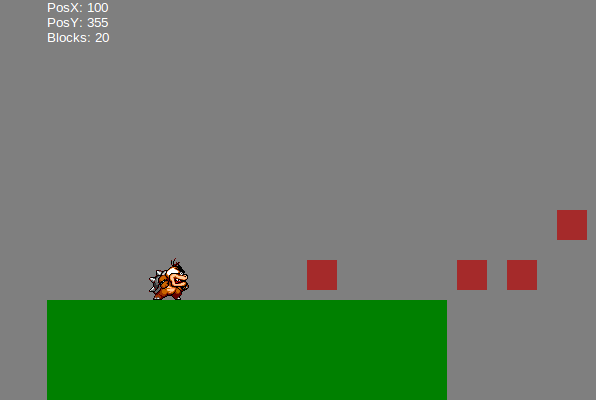
\includegraphics[width=0.45\textwidth]{images/game.png}
  \caption{The final game at the start point.}
\end{figure}
\newpage

\section{Physics Engine}
A physics engine is able to recreate an entire physical system like our world. They are mostly common in animated films, scientific experiments and video games. The gravity is the biggest part to cover. There are less and more accurate engines. In some the falling objects get faster or the objects can break when they fall on a solid ground.

\subsection{Gravity Example}
A block gets thrown horizontally with the force F. This block has now the force from the throw (horizontally) and from the gravity (vertically).\bigskip\\

\begin{figure}[H]
  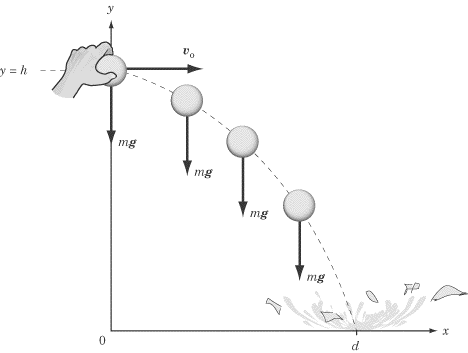
\includegraphics[width=0.45\textwidth]{images/gravity_example.png}
  \caption[Gravity example from \url{http://www.sparknotes.com/testprep/books/sat2/physics/chapter7section1.rhtml}]{Example for gravity.}
\end{figure}

\subsection{Collision Example}
A block gets thrown horizontally with the force F and collides with another, steady one with the same size and weight. After the collision the first block will fly back with half the force, while the other one gets pushed away with the other half of the force.

\begin{figure}[H]
  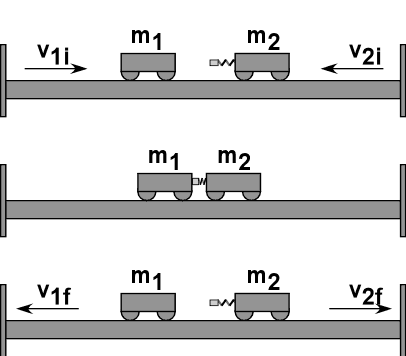
\includegraphics[width=0.45\textwidth]{images/collision_example.png}
  \caption[Collision example from \url{http://physicslearning2.colorado.edu/pira/resources/physics-testlecture-drawings}]{Example for a collision.}
\end{figure}

\subsection{Types of Physics Engines}
There are two main types of physics engines. The high-precision and the real-time engines:
\begin{description}
  \item[high-precision] This type of engine is used for exact copies of a physical system. They are mostly common for animations that must be very precise like scientific studies or animated films. It does not matter in this animations how many resources where used while rendering because you can let the machine run for many hours rendering the world and than analyze the result at the end.\smallskip\\
    To wrap it up: Those engines need much processing powers but are very precise. \ul{Quality before quantity}.
  \item[real-time] This type of engine is used for interactive animations like video games. The artificial physics must be calculated immediately. Unlike the high-precision engines this type of engine does not need much processing power, for it is minimized.\smallskip\\
    To wrap it up: The real-time engines do not need much processing power but are not very accurate. \ul{Quantity before quality}.
\end{description}

\subsection{What do we need?}
\begin{description}
  \item[collision] We need to be able to check for a collision between the player and a block above the ground.
  \item[gravity] We need to be able to use gravity to jump and fall down. 
  \item[real-time] We are creating a game, so we need in the first place a fast engine.
\end{description}
\subsection{Setting Boundaries}
But let us stop here. Even though it is a really interesting topic, it is too extensive to go into the details. If you would like to know more, there are plenty of comprehensive studies about physics engines.
\newpage

\section{Game Engine}
We want the physics engine to create a game. But how can one do this? All by himself? No, we need to find a link between the game and the physics engine. This is where the game engine has a turn. It offers the opportunity never to touch the physics engine and to make the step from a world with just moving objects to a world, controlled by a human.
\subsection{What does a Game Engine?}
\begin{itemize}
  \item It unburdens the interaction between the human's controls like a keystroke or a mouse click and the animations that can be seen on the display.
  \item It eases the animations of the objects. For example when the player walks then should the character animate this movement.
  \item It implements the element of sound. With this feature you can easily add background music and/or sound effects.
  \item They are mostly specialized on 2D or 3D worlds. 3D worlds are way more complicated but they are more realistic.
  \item They are either built for a specific platform or they can compile the same source code for multiple platforms. For example if it supports multiple platforms you can create a game and run it on Windows, Linux, Xbox and PlayStation.
  \item Some engines even include a AI system to help building one. They often helps with the data logistics and sensor access.
\end{itemize}

\subsection{Examples of Game Engines}
\begin{description}
  \item[CryENGINE] A engine created by Crytek. It runs on PS3, Xbox 360 and PC. It has an advanced AI system with sensors like sight and hearing. The games Crysis, FarCry and Warface are the most famous of many.
  \item[Unreal Engine] A engine created by Epic Games. It runs on PC, PS3, Xbox 360, Wii U, PSVITA, Android, iOS and Flash. The Unreal AI is also advanced and includes a special navigation mesh system to optimize the performance and memory usage. Dishonored, Gears of War, Batman: Arkham City and Mass Effect are the best examples for this engine.
  \item[Anvil] Until 2006 it was known as Scimitar and is created by Ubisoft. It runs on PC, PS3, Xbox 360, Wii U and PSVITA. Prince of Persia, Assassin's Creed and Tom Clancy's Rainbow 6: Patriots are the most known examples for this engine.
  \item[IW Engine] A engine created by Infinity Ward. It runs on PC, PS3, Xbox 360, Wii and Wii U. The complete Call of Duty series expect the first one is based on this engine.
  \item[Blender] This is the most popular open source game engine. 
\end{description}

\subsection{What do we need?}
We don't need a complex game engine for we are creating a simple, 2 dimensional game. It should just cover the basic necessities like:
\begin{itemize}
  \item interaction between user interface and animations
  \item animations for the objects
  \item sound implementations
  \item built for PC only should be sufficient
  \item 2 dimensional
\end{itemize}
\newpage

\section{The Game}
For it would take too much time to create an own physics and game engine, we decided to use the open source engine Crafty. It is based on the programming language JavaScript allowing the game to run in a modern web browser.

\subsection{Goal}
  We want to create a game with this specifications:
  \begin{itemize}
    \item 2 dimensional
    \item jump and run
    \item blocks to jump on
    \item gaps in the floor to fall down
    \item randomly generated
    \item generator ensures that the game is solvable
    \item finish line at the end of the parcour
    \item die from falling down
    \item win from reaching the finish line
    \item after winning or dying: restart the game
  \end{itemize}

\subsection{Basic Composition}
We used a event-driven development architecture. That means that the engine triggers events and we define what should happen.\bigskip\\
Here is the main structure of the game in a theoretically programming language:
\begin{verbatimtab}
When the player hits a solid object:
  The player stops moving

When the player hits a deadly area:
  The player dies
  Restart the game

When the player hits the finish line:
  The player wins
  Restart the game
\end{verbatimtab}


\subsection{Animation Sprites}
To bring life to our player we decided to use a sprite. A sprite is basically a collection of images with the same character but in different positions. You just have to decide which of them belong to which movement.\bigskip\\

\begin{figure}[H]
  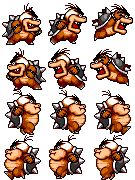
\includegraphics{images/player.png}
  \caption{The sprite to animate our player.}
\end{figure}

\begin{description}
  \item[standing right] If the player stands and looks to the right the game should use the image from \ul{row 1} and \ul{column 1}
  \item[standing left] If the player stands and looks to the left the game should use the image from \ul{row 2} and \ul{column 1}
  \item[jumping right] If the player jumps to the right the game should use the image from \ul{row 1} and \ul{column 3}
  \item[jumping left] If the player jumps to the left the game should use the image from \ul{row 2} and \ul{column 3}
  \item[walking right] If the player walks to the right the game should switch through all images from \ul{row 3}
  \item[walking left] If the player walks to the left the game should switch through all images from \ul{row 4}
\end{description}

\newpage
\subsection{Environment Creator}
Our environment consists of blocks and a floor with gaps. We now need a creator that generates random environments. To make it consistent we chose that all blocks have the same size. They are in one of this three heights:
\begin{enumerate}
  \item The height of the player. Easy to jump on.
  \item Twice the height of the player. The maximal height to jump on.
  \item Thrice the height of the player. Just reachable from a block from the first or second height.
\end{enumerate}
\begin{figure}[H]
  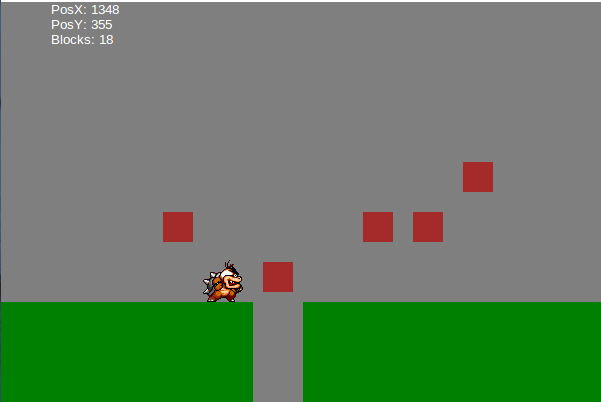
\includegraphics[width=0.45\textwidth]{images/block_heights.png}
  \caption{The three possible block heights.}
\end{figure}
The gaps in the floor exist in three different sizes:
\begin{description}
  \item[one block] These gaps are very easy to jump over.
  \item[two blocks] These are a little harder, but should pose no problem.
  \item[three blocks] These are the most difficult ones. To jump over them you have to stand on the very last corner of the floor or on a block.
\end{description}
\begin{figure}[H]
  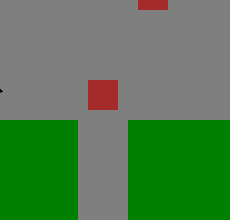
\includegraphics[width=0.145\textwidth]{images/gap_size1.png}
  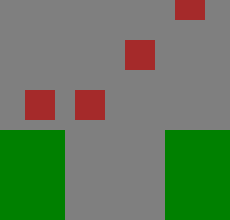
\includegraphics[width=0.145\textwidth]{images/gap_size2.png}
  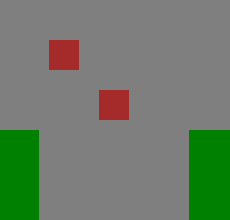
\includegraphics[width=0.145\textwidth]{images/gap_size3.png}
  \caption{The three possible sizes of the gaps.}
\end{figure}

\subsubsection{Prevent Unsolvable Environments}
Basically we could just say ``create some blocks and some gaps in the ground'' but it would most likely get unsolvable. To prevent this we have chosen this insurances to prevent that:
\begin{itemize}
  \item The blocks from the first or second height are no problem for the player to jump on.
  \item The blocks on the third height may not exist if they don't have an accessible block from the first or second height. This is to make sure that the player can jump on every block.
  \item The gaps may not be bigger than the player could jump. 
\end{itemize}

\subsubsection{Composition}
This is the basic composition of the creator in a theoretical programming language:
\begin{verbatimtab}
Define the start point
Until the whole width of the field is used:
  Set a random end point
  Create a ground from the start to end point
  Get a random gap width (1, 2 or 3)
  Set the start point: end point + gap width

15 times:
  Until the x-coordinate is unique:
    Generate random x-coordinate

  Get a random height of 1 or 2
  Generate the block from x and the height

  With a probability of 3:
    Generate a next block with the height 3
\end{verbatimtab}


\newpage
\section{Application Programming Interface (API)}
As mentioned before we need to create an interface for the AI to control the player and read the environment. To gain full control we need actors and sensors.\medskip\\
For the human the actors are the keys and his fingers with which he can handle the player. The sensors are the monitor and his eyes. With this he can analyze what is happening.\medskip\\
Now we have to adapt those actors and sensors to our API.
\subsection{Actors}
The actors are responsible for the actions of the player. We need those available actions:
\begin{description}
  \item[jump] The AI must be able to jump to the left and the right.
  \item[walk] The AI must be able to walk to the left and the right.
\end{description}

\subsection{Sensors}
The sensors are responsible for the measuring of the environment. We need those available sensors:
\begin{description}
  \item[won?] Did the player win?
  \item[died?] Did the player die?
  \item[my position] Where is the position of the player?
  \item[nearest block] Where is the nearest block?
  \item[all blocks] Where are all blocks? This is needed to plan a few steps further
  \item[nearest gap] Where is the nearest gap?
  \item[all gaps] Where are all gaps?
  \item[finish line] Where is the finish line? To check if the AI is going in to the right direction.
\end{description}

\section{Our Artificial Intelligence (AI)}


%----------------------------------------------------------------------------------------

\chapter{Sum up}


\chapter{Sources and Glossary}

\section{Sources}
\begin{description}
  \item[Physics Engines] \hfill \\
    \begin{itemize}
      \item \printhref{http://en.wikipedia.org/wiki/Physics\_engine}{Physics engine - Wikipedia}
    \end{itemize}
  \item[Game Engines] \hfill \\
    \begin{itemize}
      \item \printhref{http://en.wikipedia.org/wiki/Game\_engine}{Game engine - Wikipedia}
      \item \printhref{http://www.crytek.com/cryengine}{CryENGINE $|$ Crytek}
      \item \printhref{http://www.unrealengine.com}{Game Engine Technology by Unreal}
      \item \printhref{http://en.wikipedia.org/wiki/Anvil\_(game\_engine)}{Anvil (game engine) - Wikipedia}
      \item \printhref{http://en.wikipedia.org/wiki/IW\_engine)}{IW engine - Wikipedia}
    \end{itemize}
  \item[The Game] \hfill \\
    \begin{itemize}
      \item \printhref{http://craftyjs.com/}{Crafty - Javascript Game Engine}
    \end{itemize}
\end{description}

\printglossary%[type=main,title={Glossary},toctitle={Glossary}]
\addcontentsline{toc}{section}{Glossary}

\section{Image Sources}
\listoffigures

\end{document}
